\documentclass[11pt]{article}

% Define margins
\setlength{\topmargin}{-1.0cm}
\setlength{\oddsidemargin}{0.1cm}
\setlength{\textwidth}{16.5cm}
\setlength{\textheight}{23.0cm}

% Packages
\usepackage{url}
\usepackage[hidelinks]{hyperref}
\usepackage{subfig}
\usepackage{graphicx}
\usepackage{comment}

% Color
\usepackage{xcolor}
\newcommand{\magenta}[1]{\textcolor{magenta}{#1}}
\newcommand{\red}[1]{\textcolor{red}{#1}}
\newcommand{\blue}[1]{\textcolor{blue}{#1}}
\newcommand{\green}[1]{\textcolor{green}{#1}}



\begin{document}
	\noindent\huge \textbf{Research Statement} \\
	\vspace{0.1em}\\
	\Large \textbf{Bishwamittra Ghosh}
		
	\normalsize
	\noindent Ph.D.\ Candidate\\
	School of Computing\\
	National University of Singapore (NUS)\\
	\blue{\url{https://bishwamittra.github.io}}



	\paragraph{}
	My research interest is on the fairness and interpretability in machine learning applied in safety-critical domains. Traditional machine learning, specifically deep learning, is infamous for its unfair predictions towards certain demographic sensitive groups, and for providing uninterpretable black-box predictions. In my dissertation research, I design algorithms to \textit{verify fairness}~\cite{ghosh2021justicia,ghosh2022algorithmic} and \textit{identify the sources of unfairness}~\cite{ghosh2022how} and  \textit{learn interpretable classifiers}~\cite{ghosh22efficient,ghosh2019incremental,ghosh2020classification}. Prior approaches aimed at these problems are limited by either scalability or accuracy or both. To this end, I closely integrate automated reasoning, formal methods, and statistics with fairness and interpretability in machine learning for scalable and accurate solutions.
	
	
	
%	In my doctoral dissertation, I have focused the fairness and interpretability aspects of machine learning.  Particularly, we have proposed algorithmic frameworks for \emph{verifying the fairness of classifiers}~\cite{ghosh2021justicia,ghosh2022algorithmic}, \emph{identifying sources of the unfairness of classifiers}~\cite{ghosh2022how}, and \emph{designing efficient interpretable classifiers}~\cite{ghosh22efficient,ghosh2019incremental,ghosh2020classification}. Fairness verification provides a formal certificate of whether a classifier achieves the desired level of fairness on specified data distribution. For identifying the sources of unfairness, we compute fairness influence functions of input features as their contribution towards the bias of the classifier. In interpretable machine learning, we efficiently learn interpretable rule-based classifiers alternative to black-box classifiers. In particular, we propose a scalable learning framework through incremental learning to learn accurate and small interpretable classification rules while enabling learning on large datasets.
	
	
	My research has thrived through multiple collaborations and internships in industry and academia. Beyond fairness and interpretability, I have collaborated on solving research problems on  group testing~\cite{ciampiconi2020maxsat} and social-spacial group queries~\cite{ghosh2018flexible,apon2021social}. We have published our works at premier conferences and journals in artificial intelligence and machine learning (AAAI-$ 2022, 2021, 2020 $, JAIR-$ 2022 $, ECAI-$ 2020 $, AIES-$ 2019 $) and databases (VLDB-$ 2018 $, TSAS-$ 2022 $).
	
	
	
	
	
	\section*{Dissertation Research}
	
	\subsection*{Research Thrust 1: Fairness in Machine Learning}
	
	Fairness in machine learning centers on detecting and mitigating bias towards different sensitive groups in the data induced by the classifier. In recent years, fairness literature is bestowed with multiple fairness definitions and algorithms to quantify and improve fairness. However, there has been insignificant progress in formally verifying multiple fairness definitions and algorithms in a framework and in identifying the sources of unfairness/bias as a pave way to design better fairness algorithms. My research goal is to assess the fairness claim of a classifier by proposing a formal fairness verification framework. Furthermore, I dive into identifying the sources of unfairness of classifiers.
	
	\subsubsection*{Probabilistic Fairness Verification} The problem in probabilistic fairness verification is to verify the bias of a classifier given the distribution of input features. The early works on fairness verification focused on measuring fairness metrics of a classifier for a given dataset. Naturally, such techniques were limited in enhancing the confidence of users for wide deployment. Consequently, recent verifiers seek to achieve verification beyond  finite dataset and in turn focus on the  probability distribution of features. More specifically, the input to the probabilistic fairness verifier is a classifier and  the distribution of features, and the output is an estimate of fairness metrics that the classifier obtains given the distribution.
	
	
%	In order to solve the fairness verification problem, existing works have proposed two principled approaches.	Firstly,~\cite{albarghouthi2017fairsquare} propose a formal method approach to reduce the verification problem into the weighted volume computation of an SMT formula. Secondly,~\cite{bastani2019probabilistic} propose a sampling approach that relies on extensively enumerating the conditional probabilities of prediction given different sensitive features and thus, incurs high computational cost. Additionally, existing works assume feature independence of non-sensitive features and consider correlated features within a limited scope, such as conditional probabilities of non-sensitive features w.r.t. sensitive features and ignore correlations among non-sensitive features. As a result, the \textit{scalability} and \textit{accuracy} of existing  verifiers remains a major challenge.
	
	
	\paragraph{Formal Fairness Verification.} In our research, we propose an efficient fairness verification framework for two classes of machine learning classifiers, classifiers represented as Boolean formulas~\cite{ghosh2021justicia} and linear classifiers~\cite{ghosh2022algorithmic}. Based on stochastic satisfiability (SSAT), our proposed verifier, called $ \mathsf{Justicia} $, verifies the fairness of Boolean classifiers such as decision trees by solving appropriately designed SSAT formulas. $ \mathsf{Justicia} $ also extends verification to compound sensitive groups, which are a combination of multiple categorical sensitive features such as race $ \in $ \{White, Black\} and gender $ \in $ \{male, female\}. Because SSAT encoding allows separate quantification to each sensitive feature without restricting the number of features. In experiments, $ \mathsf{Justicia} $ is more scalable than the existing SMT and sampling-based probabilistic verifiers, and more robust than the sample-based empirical verifiers. We also prove a finite-sample error bound on estimated fairness metrics, which is stronger than the existing asymptotic guarantees.
	
	
	\paragraph{Tractable Fairness Verification.} Linear classifiers have attracted significant attention from researchers in the context of fair algorithms. Existing fairness verifier suffers from two-fold limitations for verifying linear classifiers: (i) poor scalability due to applying SSAT/SMT or sampling-based techniques and (ii) inaccuracy due to ignoring feature correlations. Consequently, we extend $ \mathsf{Justicia} $ to accurately and scalably verify linear classifiers. In this extension, we propose verification based on novel \textit{stochastic subset-sum problem}, which obtains pseudo-polynomial complexity using dynamic programming. To address feature correlations, we consider a graphical model, particularly a Bayesian Network, that represents conditional dependence (and independence) among features in the form of a DAG (directed acyclic graph). Experimentally,  $ \mathsf{Justicia} $ is more accurate and scalable than existing fairness verifiers for linear classifiers; $ \mathsf{Justicia} $ can verify group and causal fairness metrics for multiple fairness algorithms. We also demonstrate two novel applications of $ \mathsf{Justicia} $ as a fairness verifier: (a) detecting fairness attacks, and (b) computing the impact of a subset of features on shifting the incurred bias of the classifiers from the original bias.
	
	
	
	
	
	
	\subsubsection*{Identification of Sources of Unfairness}
	While fairness metrics globally quantify bias, they cannot detect or explain the sources of bias. To identify the sources of bias and also the effect of affirmative/punitive actions to alleviate/deteriorate bias, it is important to understand \textit{which factors contribute how much to the bias of a classifier on a dataset}. To this end, we follow a feature-attribution approach to understand the sources of bias, where we relate the \emph{influences} of input features towards the resulting bias of the classifier. Particularly, we define and compute \textit{Fairness Influence Function} (FIF) that quantifies the contribution of an individual and a subset of features to the resulting bias~\cite{ghosh2022how}. FIFs not only allow practitioners to identify the features to act upon but also to quantify the effect of various affirmative or punitive actions on the resulting bias. Relying on global sensitivity analysis, we instantiate an algorithm, $ \mathsf{FairXplainer} $, that uses variance decomposition among the subset of features and a local regressor to compute FIFs accurately, while also capturing the intersectional effects of the features. Our experimental analysis validates that $ \mathsf{FairXplainer} $ captures the influences of both individual features and higher-order feature interactions, estimates the bias more accurately than existing local explanation methods, and detects the increase/decrease in bias due to affirmative/punitive actions in the classifier.
	
	
%	\paragraph{Fairness Influence Functions.} Our next research quest is to \emph{quantify the influence of different features on the incurred bias of a classifier on a dataset}~\cite{ghosh2022how}. To this end, we propose a framework of Fairness Influence Function (FIF), and compute it as a scaled difference of the conditional variances in the classifier’s prediction. Based on global sensitivity analysis (GSA), we instantiate an algorithm, $ \mathsf{FairXplainer} $, that uses variance decomposition among the subset of features and a local regressor to compute FIFs accurately, while also capturing the intersectional effects of the features. Our experimental analysis validates that FairXplainer captures the influences of both individual features and higher-order feature interactions, estimates the bias more accurately than existing local explanation methods (Figure~\ref{fig:estimation_error}), and detects the increase/decrease in bias due to fairness affirmative/punitive actions in the classifier.
	
	
	\begin{comment}
	\begin{figure*}[t!]
		\begin{minipage}{0.45\textwidth}
			\centering
			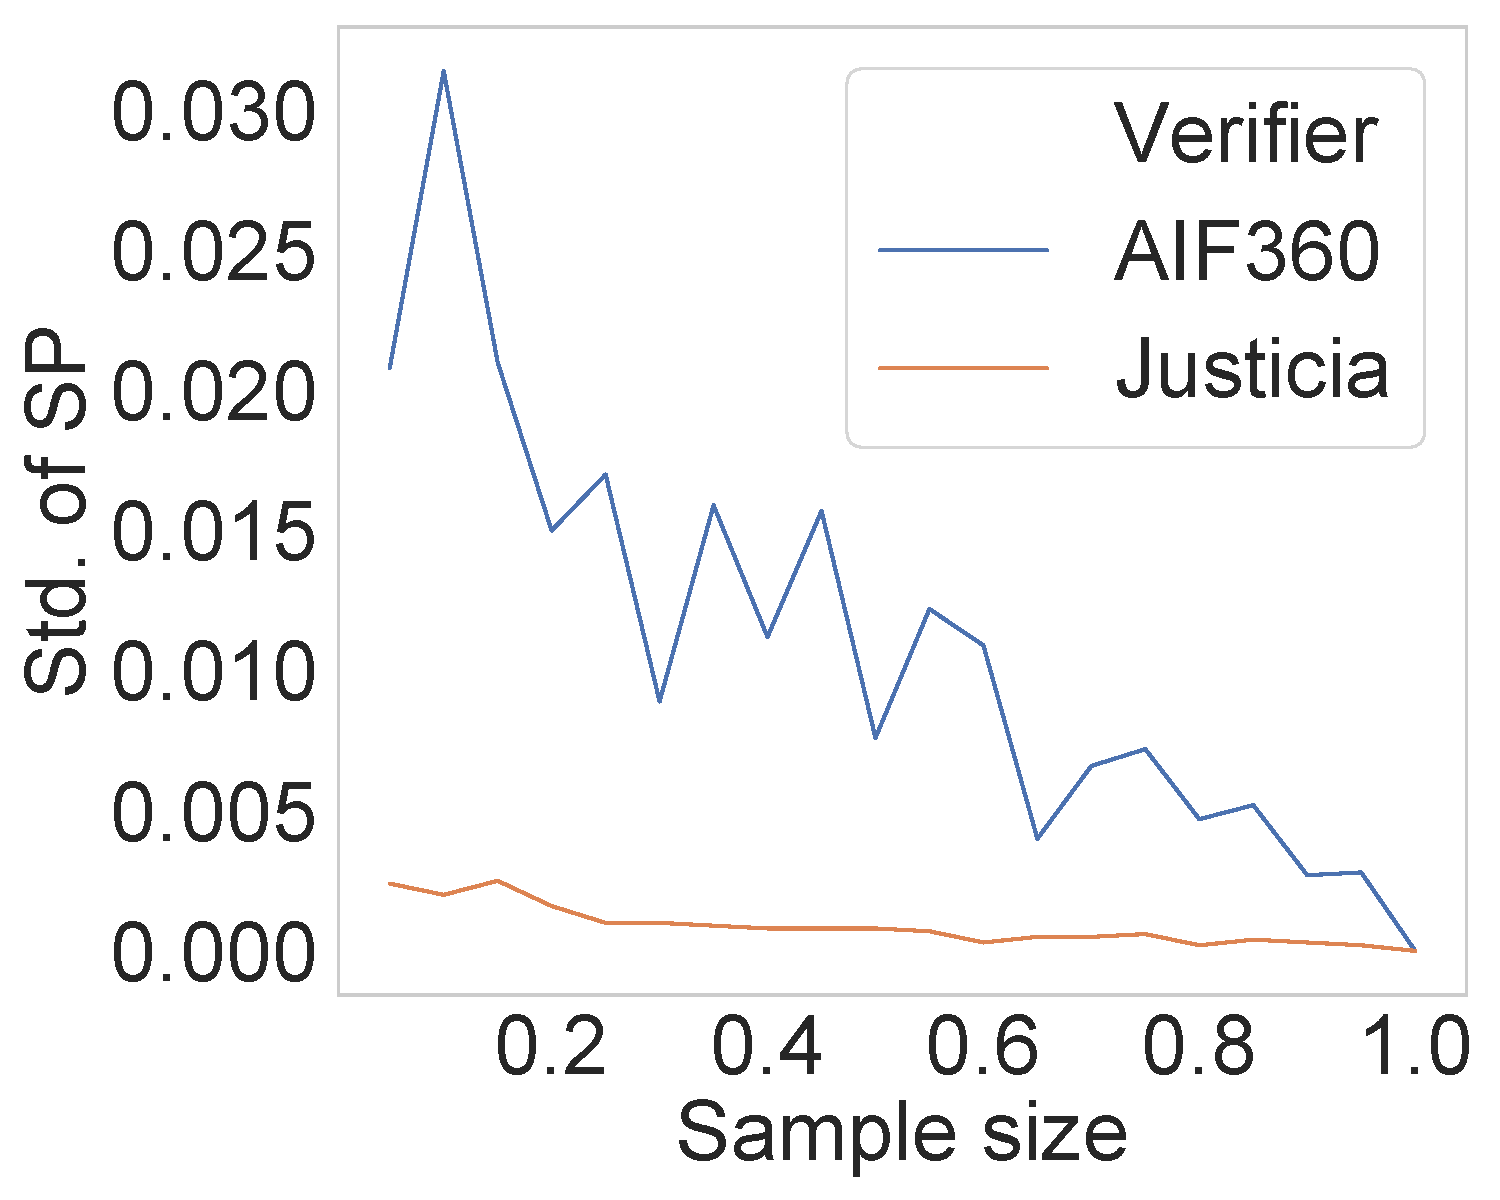
\includegraphics[scale=.18]{figures/sampling_SPD_after_Adult_rw_LR_race.pdf}
			\caption{Standard deviation in the estimation of statistical parity (SP)  for different sample sizes (sample size $ = 1 $ denotes the entire dataset). Probabilistic verifier $ \mathsf{Justicia} $ is more robust with the variation in sample size than AIF360 estimating statistical parity on a finite dataset. }
			\label{fig:sample-size}
		\end{minipage}\hfill
		\begin{minipage}{0.48\textwidth}
			\centering
				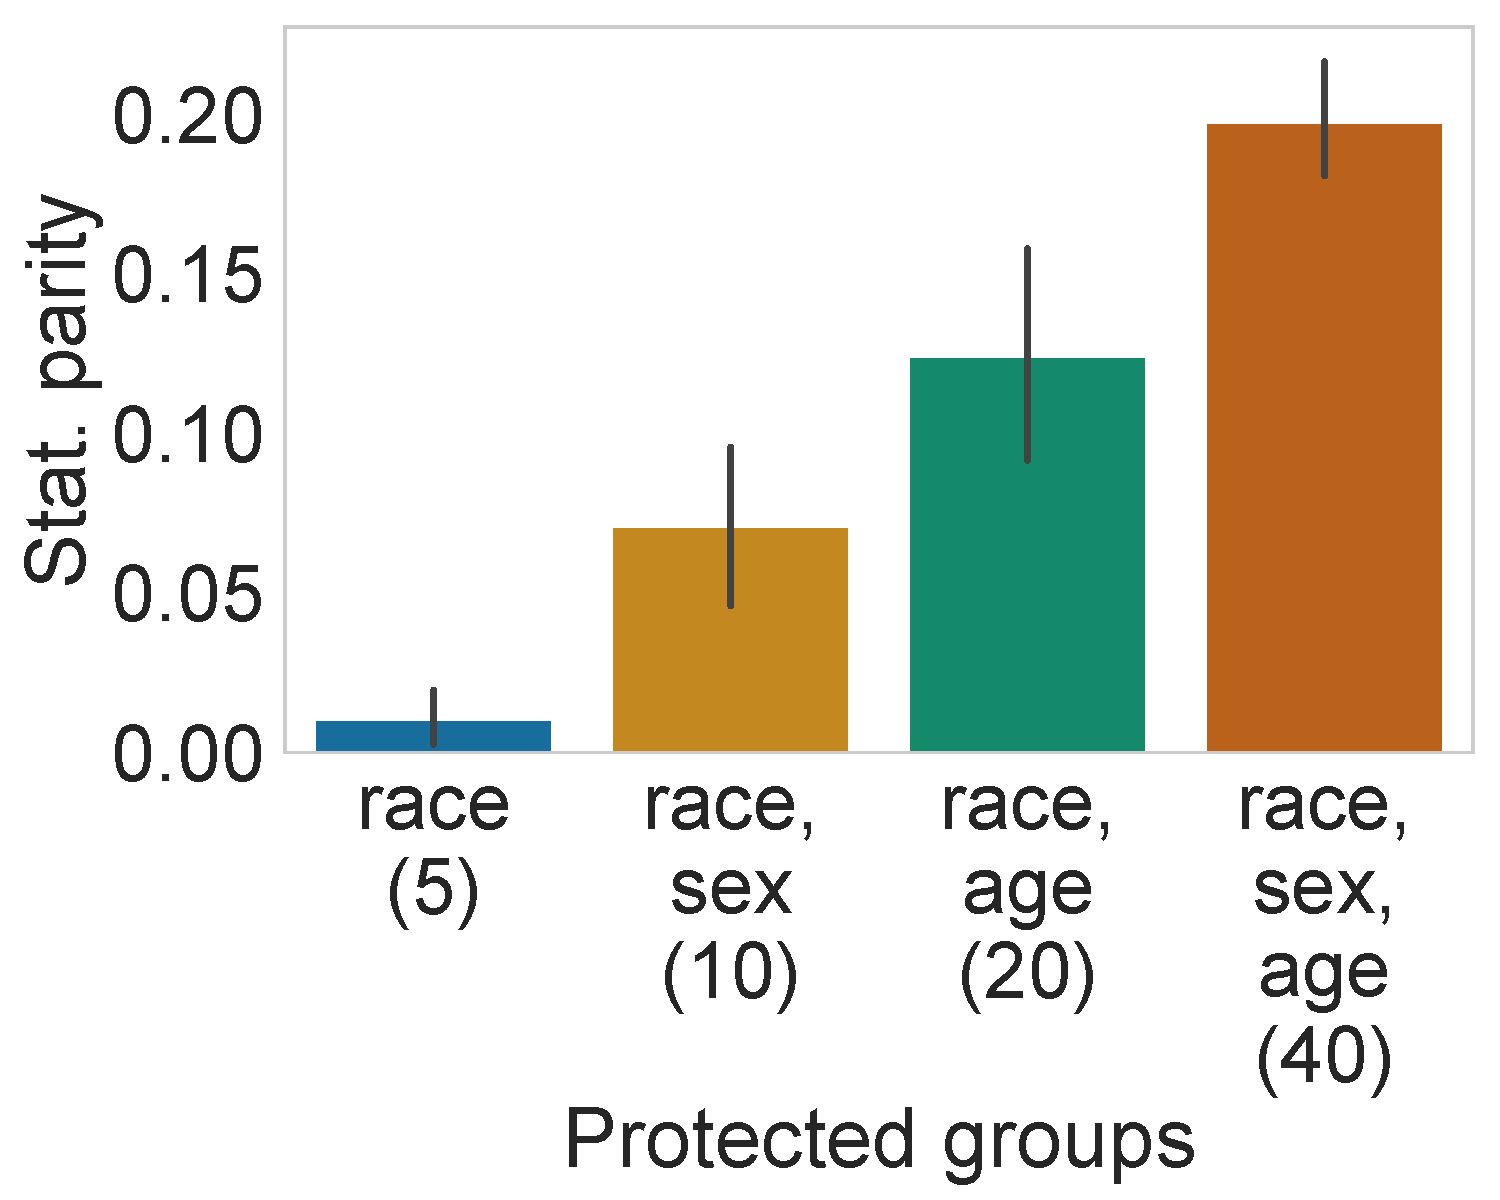
\includegraphics[scale=.18]{figures/sensitive_attribute_race_spd_Adult_DT_RE.pdf}
			\caption{Statistical parity verified by $ \mathsf{Justicia} $ for different sensitive/protected groups in the Adult dataset. The number within parenthesis in the xticks denotes total compound sensitive groups. The classifier demonstrates more unfairness (higher statistical parity) when considering more groups.}
			\label{fig:protected_groups}
		\end{minipage}
	\end{figure*}
	
	
	
	\begin{figure}
		\begin{minipage}{0.47\textwidth}
			\centering\begin{center}		
			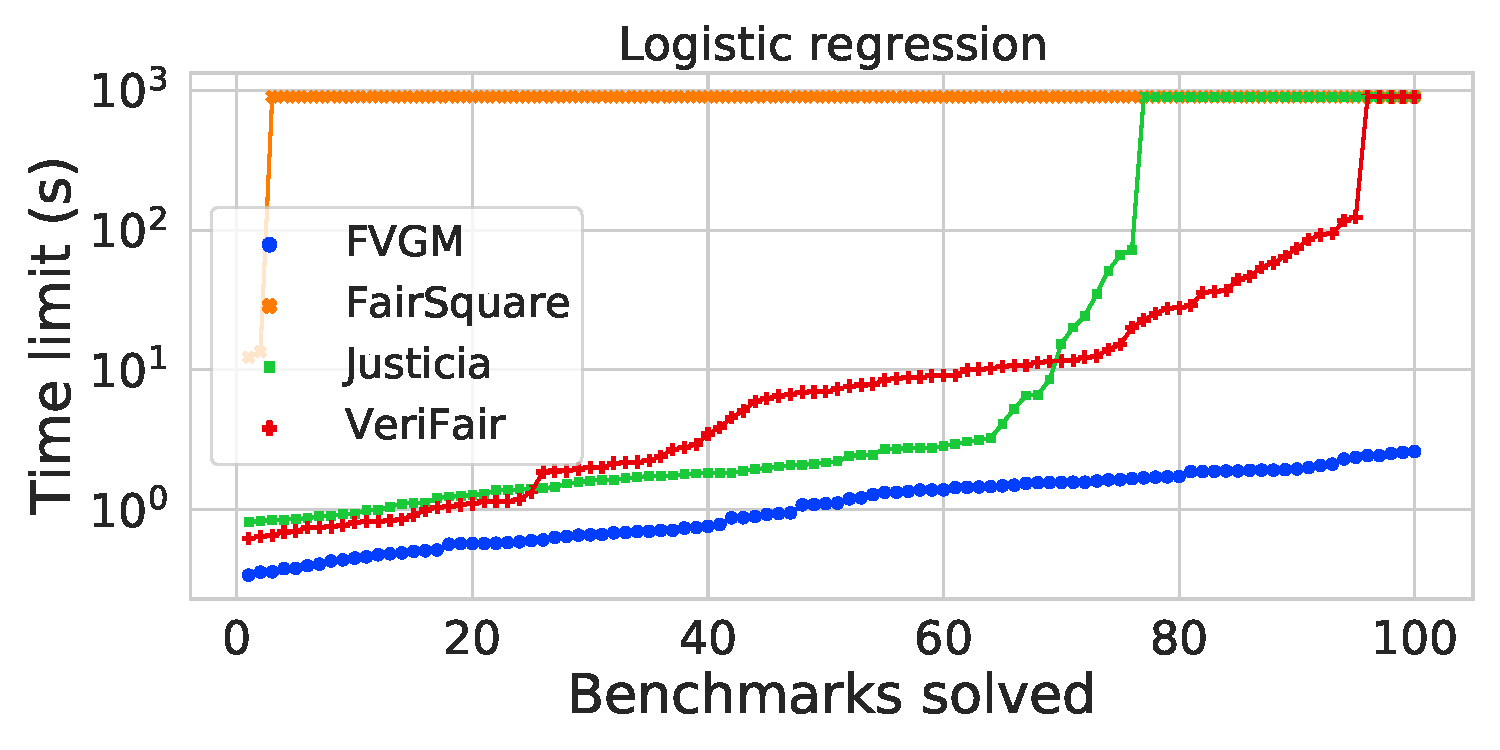
\includegraphics[scale=0.3]{figures/cactus_all_verifiers_LR_time_}
			\end{center}
			\caption{A cactus plot to present the scalability of different fairness verifiers in solving $ 100 $ fairness verification benchmarks. $ \mathsf{FVGM} $ achieves the best scalability results by solving all benchmarks with $ 1 $ to $ 2 $ orders of runtime improvement.} \label{fig:scalability_exp}
		\end{minipage}\hfill
		\begin{minipage}{0.48\textwidth}
			\centering
			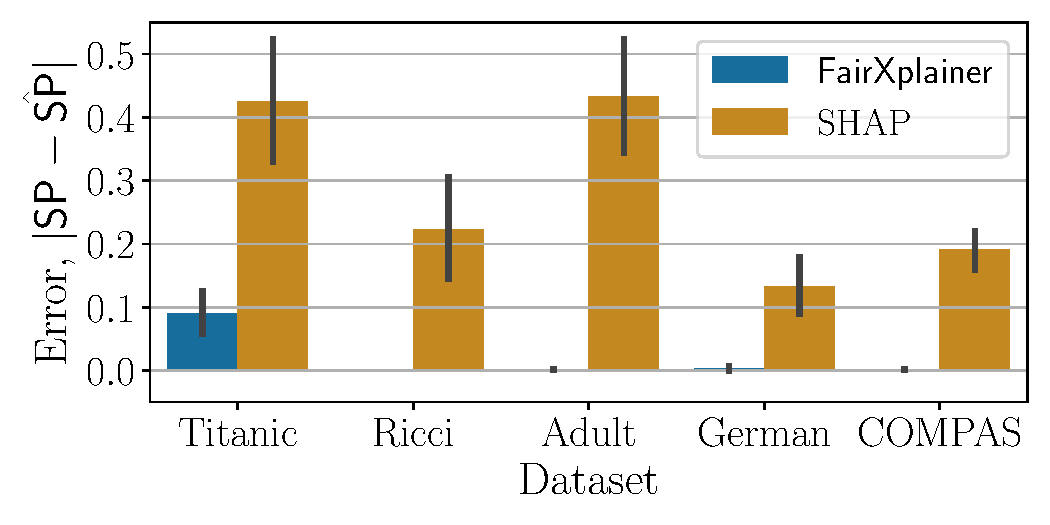
\includegraphics[scale=0.4]{figures/sp_train_accuracy}
			\caption{Comparing $ \mathsf{FairXplainer} $ and local explanation method SHAP on the estimation error of statistical parity, computed as the sum of FIFs of all subset of features~\cite{ghosh2022how}. Lower values on the $ Y $-axis denote a better result. $ \mathsf{FairXplainer} $ has significantly less estimation error than SHAP.}\label{fig:estimation_error}
		\end{minipage}
		%	\vspace{-0.5em}
	\end{figure}
	\end{comment}
	
	
	
	\subsection*{Research Thrust 2: Interpretable Machine Learning}

	In interpretable machine learning, rule-based classifiers are particularly effective in representing the decision boundary using a set of rules. The interpretability of rule-based classifiers is generally related to the size of the rules, where smaller rules with higher accuracy are preferable in practice. As such, interpretable classification learning becomes a combinatorial optimization problem suffering from poor scalability in large datasets. To this end, we propose an \textit{incremental learning framework} to extend interpretable classification to large datasets by wrapping MaxSAT (maximum satisfiability) and MILP (mixed integer linear programming) solving in mini-batch learning.
	
	\subsubsection*{Scalability via Incremental Learning}
	We propose an incremental learning framework, called $ \mathsf{IMLI} $~\cite{ghosh22efficient,ghosh2019incremental},  based on MaxSAT for synthesizing interpretable classification rules expressible in proposition logic. $ \mathsf{IMLI} $ considers a joint objective function to optimize the accuracy and the interpretability of classification rules and learns an optimal rule by solving an appropriately designed MaxSAT query. Despite the progress of MaxSAT solving in the last decade, the straightforward MaxSAT-based solution cannot scale to practical classification datasets containing thousands to millions of samples. Therefore, we incorporate an efficient incremental learning technique inside the MaxSAT formulation by integrating mini-batch learning and iterative rule-learning. The resulting framework learns a classifier by iteratively covering the training data, wherein in each iteration, it solves a sequence of smaller MaxSAT queries corresponding to each mini-batch. In our experiments, $ \mathsf{IMLI} $ achieves the best balance among prediction accuracy, interpretability, and scalability. For instance, $ \mathsf{IMLI} $ attains a competitive prediction accuracy and interpretability w.r.t.\ existing interpretable classifiers and demonstrates impressive scalability on large datasets where both interpretable and non-interpretable classifiers fail. As an application, we deploy $ \mathsf{IMLI} $ in learning popular interpretable classifiers such as decision lists and decision sets.
	
	\subsubsection*{Expressiveness via Logical Relaxation}
	We extend our incremental learning framework to learn a more relaxed representation of classification rules obtaining higher expressiveness~\cite{ghosh2020classification}. Elaborately, we consider relaxed definitions of standard OR/AND operators in Boolean logic, which allow exceptions in the construction of a clause and also in the selection of clauses in a rule. Building on these relaxed definitions, we introduce relaxed logical classification rules \textit{motivated by the popular usage of checklists in the medical domain and Boolean cardinality constraints in logic}. Relaxed logical classification rules generalize widely employed rule representations including CNF, DNF, and decision sets. While the combinatorial structure of these rules offers exponential succinctness, the na\"ive learning techniques are computationally expensive. To this end, we propose an incremental mini-batch learning procedure, called $ \mathsf{CRR} $, that employs advances in MILP solvers to efficiently learn such rules. Our experimental analysis demonstrates that $ \mathsf{CRR} $ can generate  more accurate and sparser classification rules compared to the alternative rule-based models.
	
	
	
	
%	\paragraph{Incremental Learning of Interpretable Classfication Rules.} We propose an incremental learning framework, called $ \mathsf{IMLI} $~\cite{ghosh22efficient,ghosh2019incremental},  based on maximum satisfiability (MaxSAT) for synthesizing classification rules expressible in proposition logic. $ \mathsf{IMLI} $ considers a joint objective function to optimize the accuracy and the interpretability of classification rules and learns an optimal rule by solving an appropriately designed MaxSAT query. Despite the progress of MaxSAT solving in the last decade, the straightforward MaxSAT-based solution cannot scale to practical classification datasets containing thousands to millions of samples. Therefore, we incorporate an efficient incremental learning technique inside the MaxSAT formulation by integrating mini-batch learning and iterative rule-learning. The resulting framework learns a classifier by iteratively covering the training data, wherein in each iteration, it solves a sequence of smaller MaxSAT queries corresponding to each mini-batch. In our experiments, $ \mathsf{IMLI} $ achieves the best balance among prediction accuracy, interpretability, and scalability. For instance, $ \mathsf{IMLI} $ attains a competitive prediction accuracy and interpretability w.r.t. existing interpretable classifiers and demonstrates impressive scalability on large datasets (Figure~\ref{fig:scalability_imli}) where both interpretable and non-interpretable classifiers fail. As an application, we deploy $ \mathsf{IMLI} $ in learning popular interpretable classifiers such as decision lists and decision sets.
	
	\begin{comment}
	\begin{figure}[!b]
		
		\centering
		
		\subfloat[Samples: $ 32,561 $\\Features: $ 94 $]{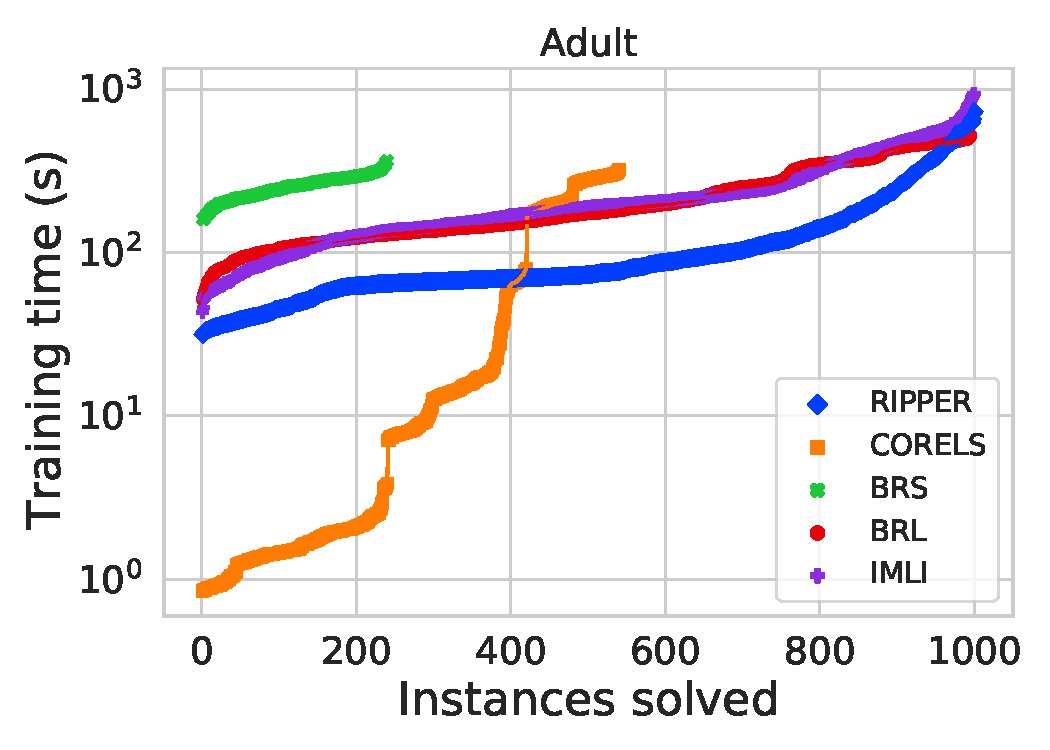
\includegraphics[scale=0.3]{figures/dataset_adult_cactus_train_val_fit_time}}
		\subfloat[Samples: $  107, 696 $\\Features: $ 169 $]{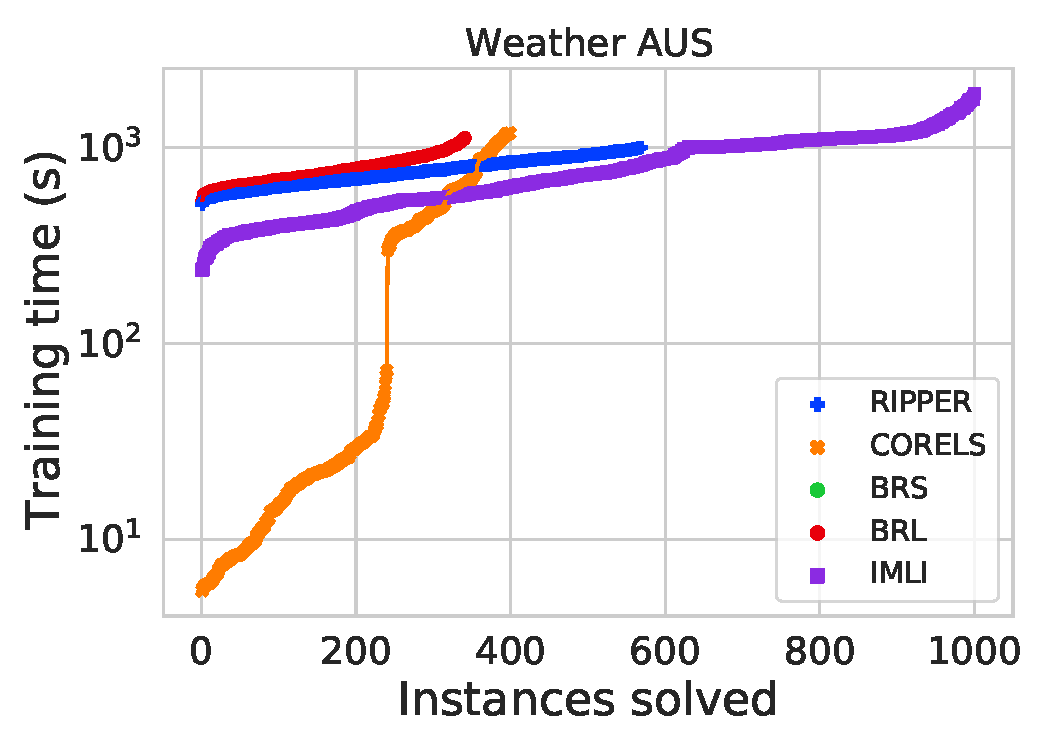
\includegraphics[scale=0.3]{figures/dataset_weatherAUS_cactus_train_val_fit_time}}
		\subfloat[Samples: $  1, 000, 000 $\\Features: $ 89 $]{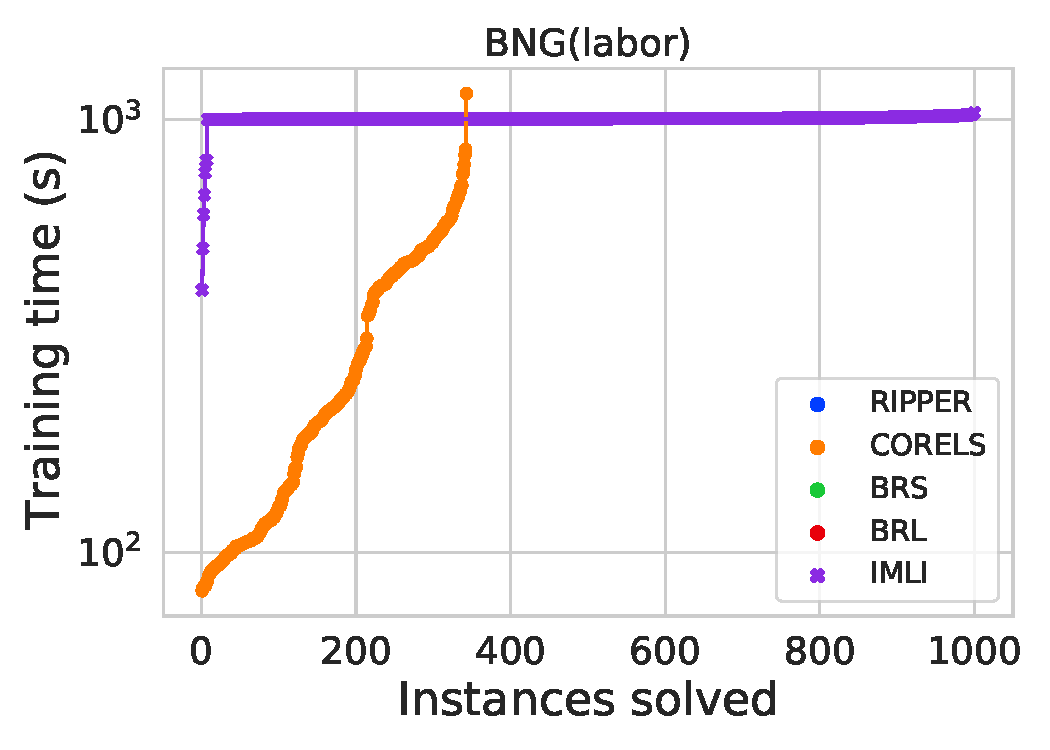
\includegraphics[scale=0.3]{figures/dataset_labor_cactus_train_val_fit_time}}
		
		\caption{Results on the scalability of $ \mathsf{IMLI} $ compared to existing interpretable classifiers, presented using cactus plots for datasets with varied dimensions. As datasets become large, $ \mathsf{IMLI} $ becomes the only interpretable classifier to classify all of $ 1000 $ classification instances for a dataset. The success of $ \mathsf{IMLI} $ is attributed to its incremental learning wrapping a MaxSAT-based formulation.}
		\label{fig:scalability_imli}
	\end{figure}
	\end{comment}
	
	
	
%	\paragraph{Classification Rules in Relaxed Logical Form.} We extend our incremental learning framework to learn a more relaxed representation of classification rules~\cite{ghosh2020classification}. Elaborately, we consider relaxed definitions of standard OR/AND operators in Boolean logic, which allow exceptions in the construction of a clause and also in the selection of clauses in a rule. Building on these relaxed definitions, we introduce relaxed-CNF classification rules motivated by the popular usage of checklists in the medical domain. Relaxed-CNF generalizes widely employed rule representations including CNF, DNF, and decision sets. While the combinatorial structure of relaxed-CNF rules offers exponential succinctness, the na\"ive learning techniques are computationally expensive. To this end, we propose an incremental mini-batch learning procedure, called $ \mathsf{CRR} $, that employs advances in the Mixed-Integer Linear Programming (MILP) solvers to efficiently learn relaxed-CNF rules. Our experimental analysis demonstrates that $ \mathsf{CRR} $ can generate relaxed-CNF rules, which are more accurate and sparser compared to the alternative rule-based models.
	
	

	
	\section*{Future Research Plans}
	 My long-term research plan is to continue designing efficient and scalable algorithms for machine learning while prioritizing its trustworthiness in safety-critical applications. I plan to work in a collaborative environment, understand problems arising in real-world applications, and solve them with advancements in machine learning and formal methods. In the following, I discuss several research themes.
	 
	 
	 \paragraph{Fairness and Interpretability As a Service.} I envision machine learning as an alternate decision-maker of the human in the future, with applications in law, education, transportation, etc. In the high-stake and safety-critical domains, end-users expect higher transparency from black-box algorithms. Hence, achieving fairness, interpretability, robustness, and privacy are significant challenges in front of current machine learning models. While traditional machine learning such as deep learning is data-hungry, certifying and verifying properties such as fainress and interpretability will be challenging in complex models and in the presence of large data. From this vantage point, I aim to design efficient algorithms for the fairness and interpretability of deep models, transformer-based natural language processing (NLP), and computer vision. 
	 
	 
	 \paragraph{Counting and Optimization Problems.} My past research has been centering on formulating fairness and interpretability in machine learning as counting and optimization problems; and our proposed algorithms based on formal methods and incremental solving result in both higher scalability and better accuracy. In the future, I plan to apply these techniques in solving counting and optimization problems, even in areas beyond machine learning. 
	
	
	\bibliographystyle{ieeetr}		\bibliography{ref}
\end{document}